\section{Results}\label{sec:results}

% Question to Denis: how exactly do you extract the IP from the XPS spectrum?
%{\color{blue}
%THESE RESULTS ARE ALREADY reported in the other paper, so we don't need them here, do we?
%
%The ionization potentials (IP) of Cl$^{-}$1s and K$^{+}$1s were measured by XPS at $h\nu = 5$\,keV, far enough from the threshold to minimize PCI effects, and calibrated on the O1s (liquid) binding energy taken at 538.1\,eV \citep{winter06:1176}. We found the value of 2825.4\,eV for the ionization potential of Cl$^{-}$ 1s (Fig.\ \ref{fg:2dmap_cl}) and 3611.9\,eV for K$^{+}$ 1s (Fig.\ \ref{fg:2dmap_k}). The full width half-maximum of these main lines was extracted and their Lorentzian contribution was measured at 0.72\,eV for K$^{+}$1s(aq) and 0.62\,eV for Cl$^{-}$1s(aq). This result agrees well with the corresponding theoretical values of 0.74\,eV and 0.64\,eV for bare potassium and chloride taken from Ref.\ \citep{Krause79:329}. In the X-ray energy region of the ionization potential of aqueous Cl$^{-}$, the photon bandwidth provided by the double crystal monochromator is about {\color{red}0.4\,eV}, whereas in the region of the ionization potential of aqueous K$^{+}$, the photon bandwidth is about {\color{red}0.5\,eV}.}


In this section we discuss the experimental results presented as 2D maps showing the dependence of the kinetic energy of the Auger electrons on the photon energy scanned across the K-edges of the aqueous potassium (Fig.\ \ref{fg:2dmap_k}) and chloride ions (Fig.\ \ref{fg:2dmap_cl}), 3611.9\,eV and 2825.4\,eV, respectively \citep{ceolin17}. The range of electron kinetic energies of the corresponding relaxation channels is larger than 2\,keV, which corresponds to inelastic mean free paths of about 50~\AA~or more in liquid water \citep{emfiet09:45}. The energies thus allow us to probe the bulk of the sample and, moreover, they ensure that the electrons escape the liquid with a sufficient count rate.


\begin{figure}%[h!]
\centering
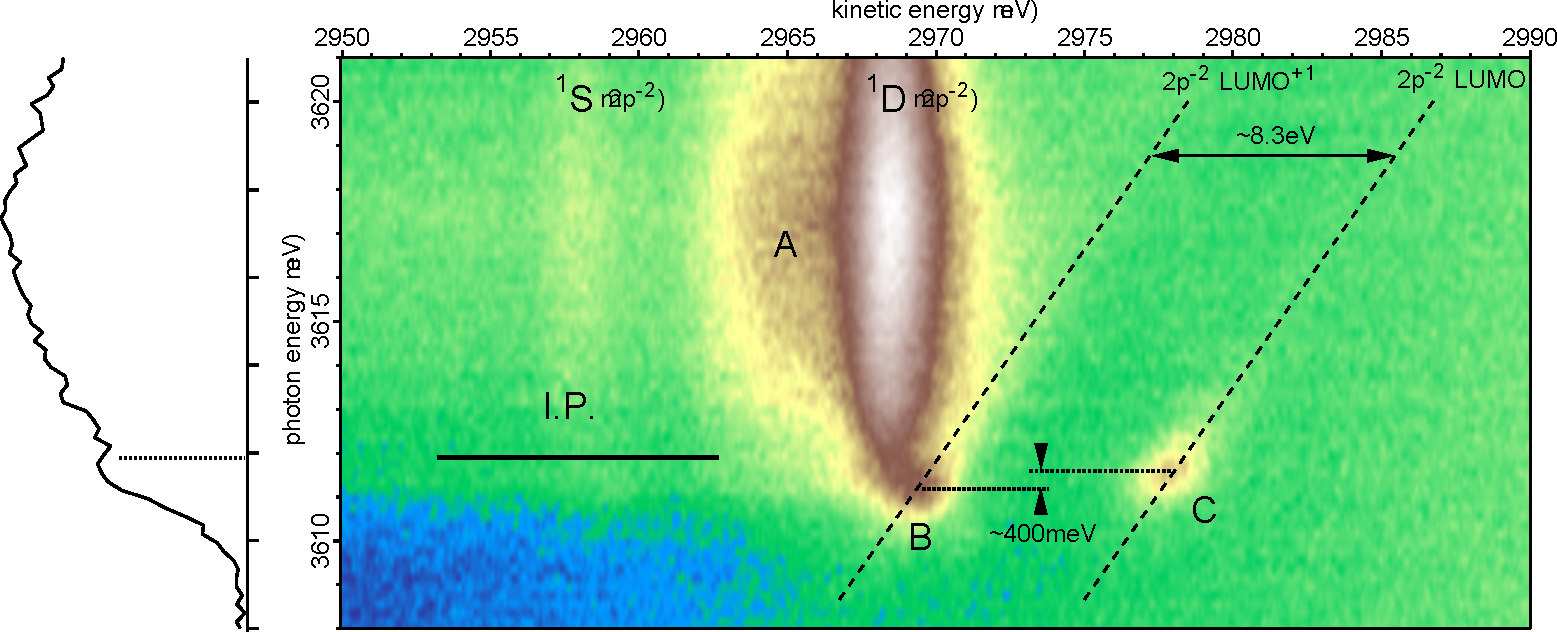
\includegraphics[scale=0.55]{figures/2Dmap_K1s_XAS.pdf}
\caption{2D map showing the kinetic energy of the electrons emitted in $K L_{2,3}L_{2,3}$ Auger decay vs the photon energy in the vicinity of the K-edge of aqueous K$^{+}$. The black curve on the left represents the experimental partial electron yield spectrum of K$^{+}$ obtained after integrating over the kinetic energies of the Auger electrons.\\
{\color{red}\bf @Denis, can you please add the letters B and C on the 2D map, and also make the 2D maps of \ki~and \cli~the same size and use the same font size?}}
\label{fg:2dmap_k}
\end{figure}


\begin{figure}%[h]
\centering
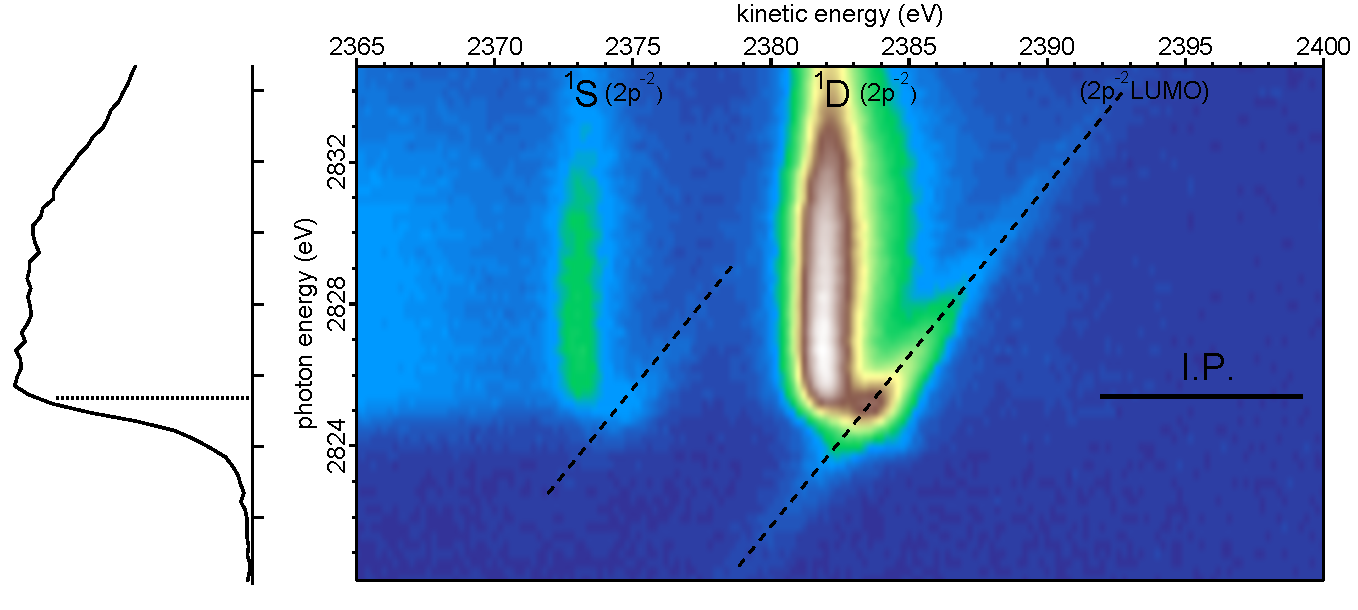
\includegraphics[scale=0.65]{figures/2Dmap_Cl1s_XAS.pdf}
\caption{2D map showing the kinetic energy of the electrons emitted in $K L_{2,3}L_{2,3}$ Auger decay vs the photon energy in the vicinity of the K-edge of aqueous Cl$^{-}$. The black curve on the left represents the experimental partial electron yield spectrum of Cl$^{-}$ obtained after integrating over the kinetic energies of the Auger electrons.}
\label{fg:2dmap_cl}
\end{figure}


\subsection{Normal Auger decay}\label{ssec:na}

Let us first consider the vertical lines at photon energies $h\nu = 3617$\,eV {\color{red}(spectrometer resolution)} on Fig.\ \ref{fg:2dmap_k} and $h\nu = 2830$\,eV {\color{red}(spectrometer resolution)} on Fig.\ \ref{fg:2dmap_cl}, respectively. They originate from KL$_{2,3}$L$_{2,3}$ Auger decay following the core ionization of K$^+$ and Cl$^-$, which leads to the population of $^3P$, $^1D$, and $^1S$ $2p^{-2}$ final states
%
\begin{align*}
h\nu + \text{K}_\text{aq}^{+} \rightarrow \text{K}_\text{aq}^{++}(1s^{-1}) + e^{-}_{\text{ph}}
			 \rightarrow \text{K}_\text{aq}^{3+} (2p^{-2}\ \ ^3P,\ ^1D,\ ^1S) + e^{-}_{\text{ph}} + e^{-}_{\text{Auger}} \\
h\nu + \text{Cl}_\text{aq}^{-} \rightarrow \text{Cl}_\text{aq}^{0}(1s^{-1}) + e^{-}_{\text{ph}}
			 \rightarrow \text{Cl}_\text{aq}^{+} (2p^{-2}\ \ ^3P,\ ^1D,\ ^1S) + e^{-}_{\text{ph}} + e^{-}_{\text{Auger}} 
\end{align*}
%
In the case of Cl$^{-}_{\text{aq}}$, the lines corresponding to the Cl$^{+}$ (2p$^{-2}$) $^1$S, $^1$D and $^3$P states are located at 2373.2\,eV, 2382.1\,eV and $\sim$2390\,eV kinetic energy. The position of the $^{3}$P line is determined approximately as the line is obscured by the dispersive feature with a maximum at 2825.2\,eV photon energy and 2383.5\,eV kinetic energy (see Fig.\ \ref{fg:2dmap_cl}). For K$^{+}_{\text{aq}}$ the maxima of the $^1$S and $^1$D KL$_{2,3}$L$_{2,3}$ Auger lines are located at 2958\,eV and 2968.4\,eV, respectively (see Fig.\ \ref{fg:2dmap_k}). The intensity of the $^3$P line is too weak and it cannot be clearly distinguished from the high-kinetic energy tail of the $^1$D line and from one of the dispersive lines with a maximum at 2969.5\,eV.


The KL$_{2,3}$L$_{2,3}$ Auger lines are not supposed to disperse with the photon energy except close to threshold due to the interaction between the photoelectron and Auger electron, i.e.\ the so-called post-collision interaction (PCI). As a result of this interaction, first, the peaks in the Auger spectrum become asymmetric with a shoulder at high kinetic energies, and second, they are shifted to higher kinetic energies close to threshold \citep{russek86:911,guillemin15:012503}. Consequently, one can attribute the high kinetic energy shoulder of the $^1$D and $^1$S peaks on Figs.\ \ref{fg:2dmap_k} and \ref{fg:2dmap_cl} as resulting from PCI effect. In order to minimize this effect we recorded the KLL Auger spectrum of both Cl$^{-}_{\text{aq}}$ and K$^{+}_{\text{aq}}$ at higher photon energies, $h\nu = 5$\,keV. The maxima of the $^3$P, $^1$D and $^1$S states were found at 2389\,eV, 2381.1\,eV and 2372.3\,eV for Cl$^{-}_{\text{aq}}$, and 2976.3\,eV, 2967.4\,eV and 2957\,eV kinetic energy for K$^{+}_{\text{aq}}$, respectively. The lines observed at a photon energy far from threshold and close to it appear to be shifted by $\sim$1\,eV. The magnitude of the shift is the same for both ions, thus, we can conclude that it does not depend on the initial charge of the ion. The observed PCI shift of 1\,eV is larger than in the case of the isoelectronic Ar, where its value is $\sim$0.5\,eV at a photon energy of 10 \,eV above threshold \citep{guillemin15:012503}. The shift in the energies of the photo- and Auger electrons is proportional to the change in the ionic field during the Auger process. In a solution, both the initial and the final Auger states will be stabilized as a result {\color{red}of ion-dipole interaction with the surrounding polarizable medium (?)}. The magnitude of this effect increases with the ionic charge. Thus, one can expect a larger change in the ionic field in an aqueous solution compared to that in a van der Waals cluster, which can, therefore, account for the large PCI shift of the Auger lines in a solution.


The normal Auger $^1$D main line of K$^{+}$ differs from that of Cl$^{-}$ by the presence of a large shoulder on the low kinetic energy side at about 2965\,eV kinetic energy. This shoulder is a result of a charge transfer process to the solvent molecules which will be the subject of a separate article \citep{ceolin17}.


\subsection{Resonant Auger decay} \label{ssec:ra}
Next, we discuss the dispersive features in the spectra of aqueous \ki~and \cli~originating from the resonant Auger decay of the core excited states below threshold. In order to get a better understanding of these features, we will first consider the Auger spectrum of the isoelectronic Ar presented in Refs.\ \citep{ceolin15:022502,guillemin15:012503}. 


First, from the 2D map of Ar one can extract information about the nature of the core excited states below threshold. The pre-edge structure in the XAS spectrum of Ar consists of the 1s$\,\rightarrow\,$4p and 1s$\,\rightarrow\,$5p excitations. Higher core excited states cannot be identified in the XAS spectrum due to their lifetime broadening and proximity to the ionization threshold. The same excitations were observed in the XAS spectrum of bare \ki~ions \citep{hertlein06:062715}. Again, the identification of 1s$\,\rightarrow\,$np states with n$> 5$ was not possible in the case of \ki.


Second, the 2D map of Ar one can extract information about the positions of the final Auger states - both in the normal and resonant Auger processes. In the case of Ar, the Ar $1s \rightarrow 4p$ and $1s \rightarrow 5p$ core excited states undergo both pure spectator and shake-up resonant Auger decay leading to the population of Ar$^{2+}(2p^{-2} np)$ ($n = 4 - 7$) final states. As a result, apart from the main Ar$^{2+}(2p^{-2})$ $^1$D and $^1$S lines which result from normal Auger decay, additional islands are observed. For example, the $1s \rightarrow 4p$ core excited state undergoes both pure spectator and shake-up resonant Auger decay. The former results in an island shifted with respect to the main $^1D$ line by $\sim$4-5\,eV kinetic energy, whereas the fingerprint of the shake-up process is a feature appearing at the same kinetic energy as the  main $^1D$ line. Moreover, the intensities of the observed shake-up features are lower compared to those of the pure spectator Auger decay. In aqueous solutions, one can expect the 2D map to be fairly different as both the initial core excited states and the final Auger states will be influenced by the presence of the solvent. 


\underline{Chloride ion Cl$^{-}$}

% 3: discussion of the dispersive lines; they are not observed in the XAS spectrum, because they overlap with the ... but they are visible on the 2D map; they result from resonant Auger decay of the 1s --> np transition in Cl-

Let us consider the features on Fig.\ \ref{fg:2dmap_cl} designated by dashed lines. Since they disperse with photon energy, they originate from Auger decay of a resonant K-shell excitation. From the 2D map we can determine the position of this core excitation at 2825.2\,eV. It is located only 0.2\,eV below the $1s$ ionization potential of Cl$^{-}_{\text{aq}}$, whose natural lifetime broadening is 0.62\,eV \citep{Krause79:329}. This state is therefore not visible in the XAS spectrum presented to the left on Fig.\ \ref{fg:2dmap_cl}, but only in a combined XAS and AES experiment. The excitation energy of 2825.2\,eV agrees very well with the position of the Cl$^{-}$ $1s \rightarrow 4p$ excitation determined by Cl K-edge XAS experiments in MgCl$_2$.6H$_2$O and of SrCl$_2$/SrCl$_2$.6H$_2$O \citep{sugiura82:681} and XXX \citep{rompel97:4465}. Contrary to the case of Ar \citep{ceolin15:022502}, with which Cl$^{-}$ is isoelectronic, a separate shake-up feature is not observed in this case.


{\color{red}
However, for atomic chloride, the description of the excited states in terms of Rydberg series is possible because the promoted electron sees an ionic core of a +1 charge. In the case of chlorine, the situation is different since the charge seen by the 1s promoted electron is null and thus using a Rydberg series description is not appropriate. More generally, it is known that isolated halide ions have no bound excited states (Berry, R. S.; Reimann, C. W.; Spokes, G. N. J. Chem. Phys. (1962), 37, 2278, Wen-Shyan Sheu and Peter J. Rossky, J. Phys. Chem. (1996), 100, 1295). However, when surrounded by water molecules, delocalized states as CTTS states have been highlighted by various MD simulations (Staib, A.; Borgis, D., J. Chem. Phys. 104, (1996), 9027 and J. Chem. Phys. 103, (1995) 2642) and experimental methods, including resonant Auger spectroscopy performed in the vicinity of the Cl-2p ionization threshold, as demonstrated by Winter et al. (JACS, 130 (2008) 7130). In the present case, we excite a s-type symmetry orbital so we expect to populate mostly p-type orbital(s). Staib, A.; Borgis, D., (J. Chem. Phys. 104, (1996), 9027 and J. Chem. Phys. 103, (1995) 2642) have calculated density of states for Cl-(aq) and highlighted a dense manifold of p-symmetry states followed by s/d symmetry states in an energy region just below the electron photo detachment threshold value, i.e., from about -1 eV to 0 eV. In our case, the 1s-1-first unoccupied state maximum is at about 0.2eV below threshold, but the corresponding core-excited state has a natural broadening of about 0.6 eV FWHM, meaning thus that the core-excited states overlap (SORRY, here again I need to add arguments).

}


\underline{Potassium ion K$^{+}$}

The calibrated (?) 2D map corresponding to the relaxation of solvated potassium ion excited in the vicinity of its K-edge is presented on Fig.\ \ref{fg:2dmap_k}. Two dispersive lines are observed in Fig.\ \ref{fg:2dmap_k}; they have maxima at $h\nu = $3611.2 \,eV and 2969.2 \,eV kinetic energy, and $h\nu = $3611.6\,eV and 2978.1\,eV kinetic energy, respectively. The first dispersive feature appears as an island, separated by approximately 8.3\,eV kinetic energy from the second dispersive feature, which on its turn is close to the $^1$D main line. Unlike in the case Cl$^{-}$ the dispersive feature close to the $^1$S main line is not found in K$^{+}$ due to presence of a strong {\color{red}BACKGROUND}.